\DiaryEntry{Cyclic Codes, I}{2017-04-18}{Coding}

\subsection{Repetition - Rings}

\begin{definition}
  A ring $(R,+,\cdot)$ is a set $R$ with two binary opeations, $+$ (addition) and $\cdot$ (multiplication), defined on $R$ such that

  \begin{itemize}
    \item $(R,+)$ forms an abelian group with additive identity typically denoted as $0$.
    \item The multiplication operation $\cdot$ is associative: $(a \cdot b) \cdot c = a \cdot (b \cdot c)$ for $a,b,c \in R$.
    \item Left and right distributive laws hold: $a(b+c) = ab + ac, (a+b)c = ac + bc$
  \end{itemize}
%
  A ring is commutative if $a \cdot b = b \cdot a$, for all $a,b \in R$. A ring is said to be a ring with identity if $\cdot$ has an identitiy element which is typically denoted as $1$.

\end{definition}

As a simple example, consider $(\mZ_6, +, \cdot)$ with addition and multiplication tables as follows (addition and multiplication are taken modulo-6):

\begin{figure}[H]
  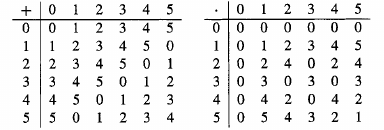
\includegraphics[scale=0.75]{images/cyclic_codes_01.png}
\end{figure}

Note that the set does not form a group under multiplication (it does under addition, though). However, this does not contradict the ring definition; i.e. the thing is a ring.


\subsection{Repetition - Rings of Polynomials}

If $R$ is a ring, then the set of all polynomials with coefficients in $R$ form a ring under the usual operations for polynomial addition and multiplication. This ring is denoted as $R[x]$, where $x$ is the polynomial variable:

\bee
f(x) = \sum_{i=0}^n a_i x^i, a_i \in R
\eee

Taking $R$ to be $(\mZ_6, +, \cdot)$, we obtain a polynomial ring as $R[x]$ with some example elements $f_1(x) = 3 + x, f_2(x) = 5 + 3x^2$. For example, we have $f_1 + f_2 = 2 + x + 3x^2$ and $f_1 f_2 = 3 + 5x + 3x^2 + 3x^3$.

\subsection{Repetition - Quotient Rings}

In Group Theory, a set of cosets was created by ``translating'' a subgroup; i.e. if $H$ is a subgroup of a group $G$, then we formed cosets by $g + H, g \in G$.

In a similar spirit, we can collect polynomials over a ring into equivalence classes by their remainder after division by a fixed polynomial.
%
As an example, consider the ring of polynomials $GF(2)[x]$ and a fixed polynomial $x^3+1$. Now collect all polynomials with remainder $0$ after division modulo $x^3+1$:

\bee
S_0 = \{0, x^3+1, x^4+x, x^5+x^2, \ldots\} = \langle x^3 + 1 \rangle
\eee
%
where $S_0 = \langle x^3 + 1 \rangle$ is the set of polynomials generated by $x^3+1$. In a similar spirit, $S_1$ contains all polynomials with remainder $1$ after division modulo $x^3+1$:

\bee
S_1 = \{1, x^3, x^4+x+1, x^5+x^2+1, \ldots\} = 1 + \langle x^3 + 1 \rangle
\eee
%
The other equivalence classes are obtained in the same manner.

\begin{figure}[H]
  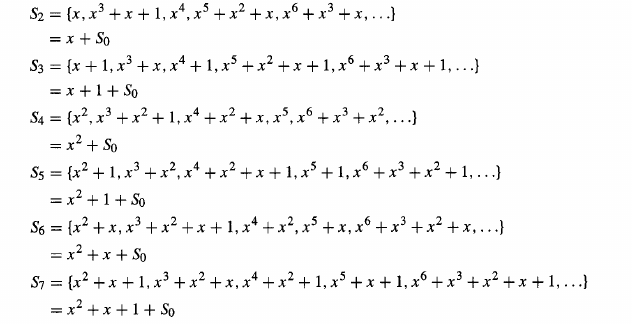
\includegraphics[scale=0.75]{images/cyclic_codes_02.png}
\end{figure}
%
By dividing through $x^3+1$, only 7 different remainders are possible: $0, 1, x, 1+x, 1+x^2, x+x^2, 1+x+x^2$. Therefore, all polynomials of $GF(2)[x]$ fall into of these equivalence classes.
%
In a similar spirit to defining an induced operation of cosets, we can define induced operations $+$ and $\cdot$ for the equivalence classes of polynomials modulo $x^3+1$ by operation on representative elements. We obtain the following tables:

\begin{figure}[H]
  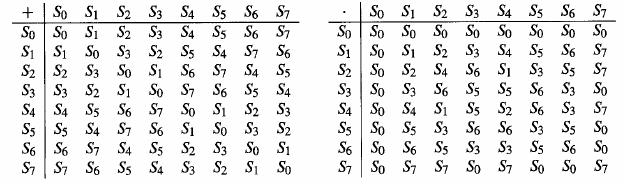
\includegraphics[scale=0.75]{images/cyclic_codes_03.png}
\end{figure}

If we define $R=\{S_0, S_1,\ldots, S_7\}$, then $(R,+)$ is an Abelian group with $S_0$ as identity and for multiplication $S_1$ acts as identity. Not every element has a multiplicative inverse, so $R - S_0$ is not a group. However, the whole thing $(R,+,\cdot)$ is a ring denoted as $GF[x]/\langle x^3+1 \rangle$.

We denote a ring $GF(2)[x]/\langle x^n-1 \rangle$ as $R_n$ and a ring $\mF_q[x]/\langle x^n-1\rangle$ as $R_{n,q}$.

\subsection{Ideals in Rings}

\begin{definition}
  Let $R$ be a ring. A nonempty subset $I \subseteq R$ is an ideal if

  \begin{itemize}
    \item $I$ forms a group under addition in $R$.
    \item For any $a \in I$ and $r \in R$, $ar \in I$.
  \end{itemize}
\end{definition}

The first point ensures that the ideal has at least some structure; i.e. adding two ideal elements yields another ideal element. The second point is interesting in that the product of an ideal and a ``non-ideal'' element is still an ideal.

As a simple example, take $R$ as the set of integers. An ideal is the set of even numbers; the sum of any two even numbers is even and the product of any number with an even one gives an even number.

\begin{definition}
  An ideal $I$ in a ring $R$ is said to be principal if there exists some $g \in I$ such that every element $a \in I$ can be expressed as a product $a = mg$ for some $m \in R$. For a principal ideal, such an element $g$ is called the generator element. The ideal generated by $g$ is denoted as $\langle g \rangle$:

  \bee
    \langle g \rangle = \{hg : h \in R\}
  \eee
  
\end{definition}

The ideal in the example above is principal with a generator element $g = 2$. Every element of the ideal can be created by $2m$ with $m \in R$.

\begin{theorem}
  Let $I$ be an ideal in $\mF_q[x] / \langle x^n-1 \rangle$. Then
  \begin{itemize}
    \item There is a unique monic polynomial $g(x) \in I$ of minimal degree.
    \item $I$ is principal with generator $g(x)$.
    \item $g(x)$ divides $(x^n-1)$ in $\mF_q[x]$.
  \end{itemize}

\end{theorem}


\subsection{Cyclic Codes}

A cyclic shift of a binary code word looks like this: We have a vector $\cbf = (c_0, c_1, \ldots,c_{n-2}, c_{n-1})$ and shift it cyclically to the right to obtain $\cbf' = (c_{n-1}, c_0, c_1, \ldots, c_{n-2})$.

\begin{definition}
  An $(n,k)$ block code is cyclic, it it is linear and if for every codeword, its right cyclic shift is also a codeword.
\end{definition}


This cyclic shifting can be expressed in terms of polynomial manipulations; If we have the codeword

\bee
\cbf = (c_0, c_1, \ldots,c_{n-2}, c_{n-1})
\eee
%
we can associate the polynomial

\bee
c(x) = \cbf = c_0 + c_1 x + c_2 x^2 + \cdots c_{n-1} x^{n-1}
\eee
%
A non-cyclic right-shift is then represented as $xc(x)$ and a cyclic right-shift is represented by $xc(x) \mod (c^n-1)$.
